\documentclass[10pt,a4paper]{amsart}
\usepackage[margin=19mm]{geometry}
\usepackage{amsmath,amssymb,mathtools}
\usepackage[scr=rsfs,cal=euler]{mathalfa}
\usepackage{xfrac}
\usepackage[unicode,hidelinks,bookmarks=false]{hyperref}
\newcommand{\ie}{i.e.\ }
\newcommand{\cf}{cf.\ }
\newcommand{\resp}{respectively\ }
\newcommand{\Subsection}{\subsection}
\providecommand{\nobreakdash}{\nobreak\hbox{-}}
\setlength{\emergencystretch}{2em}
\multlinegap0pt
\usepackage{tikz}
\usepackage{float}
\newtheorem{theorem}{Theorem}
\newcommand{\miff}{\Longleftrightarrow}
\title{Regular non-normal modal classicalities}
\author{Alfredo Roque Freire, Manuel Ant\'onio Martins}
\date{Source: arXiv:2602.20287v1 (CC BY 4.0)}
\begin{document}
\maketitle

\noindent\emph{Source and licence.} Regular non-normal modal classicalities. Version arXiv:2602.20287v1 (CC BY 4.0), distributed by arXiv under the Creative Commons Attribution 4.0 International licence, http://creativecommons.org/licenses/by/4.0/, as recorded in the arXiv licence metadata for this exact version and shown on the abstract page https://arxiv.org/abs/2602.20287v1. Full licence notice: \texttt{licenses/arxiv-2602.20287-CC-BY-4.0.txt}.\par\smallskip

\noindent\textit{Editorial scope.} Counted unit: the article's theorem soobNotCharacterizable (source0.tex lines 908--910). The article's complete original proof of it is delivered with it (source0.tex lines 912--1100, one \texttt{proof} environment of 189 lines). No mathematics is written, repaired or re-derived: the statement and the proof are the article's own lines, in the article's own notation, and no retained line is substituted or re-flowed.  No further source-local context is needed: every cross-reference of every retained line resolves inside the two delivered spans.  Nothing was omitted from any retained span, so the package carries no omission record.  No retained line contains a citation, so the wrapper carries no bibliography and no bibliography entry.  The retained lines contain the article's own diagram code, which the wrapper typesets with the standard tikz packages; no image file is delivered and the package declares no asset dependency.  Editorial formatting only, in addition: an AMS \texttt{amsart} preamble that restates the article's own declarations and macros used by the retained lines, namely the environments \texttt{theorem} on separate counters, together with the standard packages those lines need.  The retained environments print in this document as Theorem 1 in order of appearance, whereas the article prints the same items with the numbering of its own full document.  The complete native source of the article as distributed in the arXiv e-print for this exact version is bundled unchanged as \texttt{sources/195175/source0.tex}.
\begin{theorem}\label{soobNotCharacterizable}
    No formula characterizes super out of the bubble.
\end{theorem}

\begin{proof}
    We will produce a frame $F$ that is super out of the bubble and a frame $F'$ that is not, and we will show that $F \vDash \varphi$ if and only if $F' \vDash \varphi$ for every formula $\varphi$. Assuming this, suppose that there is a formula $\theta$ that characterizes super out of the bubble. Because $F$ is super out of the bubble, $F \vDash \theta$; From the equivalence, this implies $F' \vDash \theta$; since $\theta$ characterizes super out of the bubble, we conclude that $F'$ is super out of the bubble, which is a contradiction.

    Consider the following frame $F$:
    \begin{center}
        \tikzset{every picture/.style={line width=0.75pt}} %set default line width to 0.75pt        
        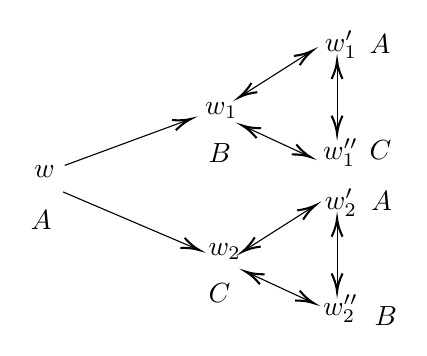
\begin{tikzpicture}[x=0.75pt,y=0.75pt,yscale=-.8,xscale=.8]
        %uncomment if require: \path (0,300); %set diagram left start at 0, and has height of 300
        
        %Straight Lines [id:da05928991953527163] 
        \draw    (185.5,185) -- (265.66,219.21) ;
        \draw [shift={(267.5,220)}, rotate = 203.11] [color={rgb, 255:red, 0; green, 0; blue, 0 }  ][line width=0.75]    (10.93,-3.29) .. controls (6.95,-1.4) and (3.31,-0.3) .. (0,0) .. controls (3.31,0.3) and (6.95,1.4) .. (10.93,3.29)   ;
        %Straight Lines [id:da10004678245610554] 
        \draw    (186.5,169) -- (260.62,141.69) ;
        \draw [shift={(262.5,141)}, rotate = 159.78] [color={rgb, 255:red, 0; green, 0; blue, 0 }  ][line width=0.75]    (10.93,-3.29) .. controls (6.95,-1.4) and (3.31,-0.3) .. (0,0) .. controls (3.31,0.3) and (6.95,1.4) .. (10.93,3.29)   ;
        %Straight Lines [id:da7434380713720259] 
        \draw    (293.19,126.93) -- (333.81,101.07) ;
        \draw [shift={(335.5,100)}, rotate = 147.53] [color={rgb, 255:red, 0; green, 0; blue, 0 }  ][line width=0.75]    (10.93,-3.29) .. controls (6.95,-1.4) and (3.31,-0.3) .. (0,0) .. controls (3.31,0.3) and (6.95,1.4) .. (10.93,3.29)   ;
        \draw [shift={(291.5,128)}, rotate = 327.53] [color={rgb, 255:red, 0; green, 0; blue, 0 }  ][line width=0.75]    (10.93,-3.29) .. controls (6.95,-1.4) and (3.31,-0.3) .. (0,0) .. controls (3.31,0.3) and (6.95,1.4) .. (10.93,3.29)   ;
        %Straight Lines [id:da10677767127325755] 
        \draw    (295.19,219.93) -- (335.81,194.07) ;
        \draw [shift={(337.5,193)}, rotate = 147.53] [color={rgb, 255:red, 0; green, 0; blue, 0 }  ][line width=0.75]    (10.93,-3.29) .. controls (6.95,-1.4) and (3.31,-0.3) .. (0,0) .. controls (3.31,0.3) and (6.95,1.4) .. (10.93,3.29)   ;
        \draw [shift={(293.5,221)}, rotate = 327.53] [color={rgb, 255:red, 0; green, 0; blue, 0 }  ][line width=0.75]    (10.93,-3.29) .. controls (6.95,-1.4) and (3.31,-0.3) .. (0,0) .. controls (3.31,0.3) and (6.95,1.4) .. (10.93,3.29)   ;
        %Straight Lines [id:da7392138944965345] 
        \draw    (295.31,145.84) -- (332.69,163.16) ;
        \draw [shift={(334.5,164)}, rotate = 204.86] [color={rgb, 255:red, 0; green, 0; blue, 0 }  ][line width=0.75]    (10.93,-3.29) .. controls (6.95,-1.4) and (3.31,-0.3) .. (0,0) .. controls (3.31,0.3) and (6.95,1.4) .. (10.93,3.29)   ;
        \draw [shift={(293.5,145)}, rotate = 24.86] [color={rgb, 255:red, 0; green, 0; blue, 0 }  ][line width=0.75]    (10.93,-3.29) .. controls (6.95,-1.4) and (3.31,-0.3) .. (0,0) .. controls (3.31,0.3) and (6.95,1.4) .. (10.93,3.29)   ;
        %Straight Lines [id:da8351408220439647] 
        \draw    (297.31,233.84) -- (334.69,251.16) ;
        \draw [shift={(336.5,252)}, rotate = 204.86] [color={rgb, 255:red, 0; green, 0; blue, 0 }  ][line width=0.75]    (10.93,-3.29) .. controls (6.95,-1.4) and (3.31,-0.3) .. (0,0) .. controls (3.31,0.3) and (6.95,1.4) .. (10.93,3.29)   ;
        \draw [shift={(295.5,233)}, rotate = 24.86] [color={rgb, 255:red, 0; green, 0; blue, 0 }  ][line width=0.75]    (10.93,-3.29) .. controls (6.95,-1.4) and (3.31,-0.3) .. (0,0) .. controls (3.31,0.3) and (6.95,1.4) .. (10.93,3.29)   ;
        %Straight Lines [id:da12403182801219348] 
        \draw    (350.5,148) -- (350.5,108) ;
        \draw [shift={(350.5,106)}, rotate = 90] [color={rgb, 255:red, 0; green, 0; blue, 0 }  ][line width=0.75]    (10.93,-3.29) .. controls (6.95,-1.4) and (3.31,-0.3) .. (0,0) .. controls (3.31,0.3) and (6.95,1.4) .. (10.93,3.29)   ;
        \draw [shift={(350.5,150)}, rotate = 270] [color={rgb, 255:red, 0; green, 0; blue, 0 }  ][line width=0.75]    (10.93,-3.29) .. controls (6.95,-1.4) and (3.31,-0.3) .. (0,0) .. controls (3.31,0.3) and (6.95,1.4) .. (10.93,3.29)   ;
        %Straight Lines [id:da6892995026591608] 
        \draw    (350.5,243) -- (350.5,203) ;
        \draw [shift={(350.5,201)}, rotate = 90] [color={rgb, 255:red, 0; green, 0; blue, 0 }  ][line width=0.75]    (10.93,-3.29) .. controls (6.95,-1.4) and (3.31,-0.3) .. (0,0) .. controls (3.31,0.3) and (6.95,1.4) .. (10.93,3.29)   ;
        \draw [shift={(350.5,245)}, rotate = 270] [color={rgb, 255:red, 0; green, 0; blue, 0 }  ][line width=0.75]    (10.93,-3.29) .. controls (6.95,-1.4) and (3.31,-0.3) .. (0,0) .. controls (3.31,0.3) and (6.95,1.4) .. (10.93,3.29)   ;
        
        % Text Node
        \draw (166.5,167.4) node [anchor=north west][inner sep=0.75pt]    {$w$};
        % Text Node
        \draw (269.5,129.4) node [anchor=north west][inner sep=0.75pt]    {$w_{1}$};
        % Text Node
        \draw (271.5,214.4) node [anchor=north west][inner sep=0.75pt]    {$w_{2}$};
        % Text Node
        \draw (341.5,86.4) node [anchor=north west][inner sep=0.75pt]    {$w'_{1}$};
        % Text Node
        \draw (340.5,151.4) node [anchor=north west][inner sep=0.75pt]    {$w''_{1}$};
        % Text Node
        \draw (340.5,245.4) node [anchor=north west][inner sep=0.75pt]    {$w''_{2}$};
        % Text Node
        \draw (341.5,181.4) node [anchor=north west][inner sep=0.75pt]    {$w'_{2}$};
        % Text Node
        \draw (164.5,194.4) node [anchor=north west][inner sep=0.75pt]    {$A$};
        % Text Node
        \draw (368.5,88.4) node [anchor=north west][inner sep=0.75pt]    {$A$};
        % Text Node
        \draw (369.5,183.4) node [anchor=north west][inner sep=0.75pt]    {$A$};
        % Text Node
        \draw (271.5,154.4) node [anchor=north west][inner sep=0.75pt]    {$B$};
        % Text Node
        \draw (371.5,252.4) node [anchor=north west][inner sep=0.75pt]    {$B$};
        % Text Node
        \draw (271.5,238.4) node [anchor=north west][inner sep=0.75pt]    {$C$};
        % Text Node
        \draw (368.5,152.4) node [anchor=north west][inner sep=0.75pt]    {$C$};
        
        
        \end{tikzpicture}
    \end{center}
    As the reader can observe, each world has the lattice $A = \{1,0,a,-a\}$, $B = \{1,0,b,-b\}$ or $C = \{1,0,c,-c\}$ written next to them. These are the lattices of each world. Now, observe that this frame is super out of the bubble. Consider then the \textbf{similar} frame $F'$:
    \begin{center}
        \tikzset{every picture/.style={line width=0.75pt}} %set default line width to 0.75pt        
        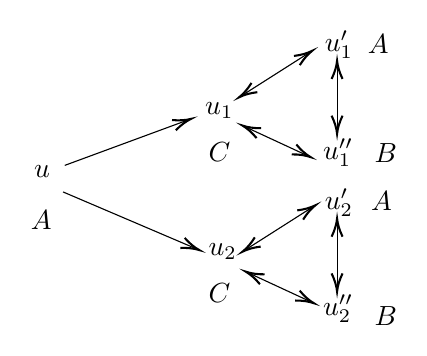
\begin{tikzpicture}[x=0.75pt,y=0.75pt,yscale=-.8,xscale=.8]
        %uncomment if require: \path (0,300); %set diagram left start at 0, and has height of 300
        
        %Straight Lines [id:da05928991953527163] 
        \draw    (185.5,185) -- (265.66,219.21) ;
        \draw [shift={(267.5,220)}, rotate = 203.11] [color={rgb, 255:red, 0; green, 0; blue, 0 }  ][line width=0.75]    (10.93,-3.29) .. controls (6.95,-1.4) and (3.31,-0.3) .. (0,0) .. controls (3.31,0.3) and (6.95,1.4) .. (10.93,3.29)   ;
        %Straight Lines [id:da10004678245610554] 
        \draw    (186.5,169) -- (260.62,141.69) ;
        \draw [shift={(262.5,141)}, rotate = 159.78] [color={rgb, 255:red, 0; green, 0; blue, 0 }  ][line width=0.75]    (10.93,-3.29) .. controls (6.95,-1.4) and (3.31,-0.3) .. (0,0) .. controls (3.31,0.3) and (6.95,1.4) .. (10.93,3.29)   ;
        %Straight Lines [id:da7434380713720259] 
        \draw    (293.19,126.93) -- (333.81,101.07) ;
        \draw [shift={(335.5,100)}, rotate = 147.53] [color={rgb, 255:red, 0; green, 0; blue, 0 }  ][line width=0.75]    (10.93,-3.29) .. controls (6.95,-1.4) and (3.31,-0.3) .. (0,0) .. controls (3.31,0.3) and (6.95,1.4) .. (10.93,3.29)   ;
        \draw [shift={(291.5,128)}, rotate = 327.53] [color={rgb, 255:red, 0; green, 0; blue, 0 }  ][line width=0.75]    (10.93,-3.29) .. controls (6.95,-1.4) and (3.31,-0.3) .. (0,0) .. controls (3.31,0.3) and (6.95,1.4) .. (10.93,3.29)   ;
        %Straight Lines [id:da10677767127325755] 
        \draw    (295.19,219.93) -- (335.81,194.07) ;
        \draw [shift={(337.5,193)}, rotate = 147.53] [color={rgb, 255:red, 0; green, 0; blue, 0 }  ][line width=0.75]    (10.93,-3.29) .. controls (6.95,-1.4) and (3.31,-0.3) .. (0,0) .. controls (3.31,0.3) and (6.95,1.4) .. (10.93,3.29)   ;
        \draw [shift={(293.5,221)}, rotate = 327.53] [color={rgb, 255:red, 0; green, 0; blue, 0 }  ][line width=0.75]    (10.93,-3.29) .. controls (6.95,-1.4) and (3.31,-0.3) .. (0,0) .. controls (3.31,0.3) and (6.95,1.4) .. (10.93,3.29)   ;
        %Straight Lines [id:da7392138944965345] 
        \draw    (295.31,145.84) -- (332.69,163.16) ;
        \draw [shift={(334.5,164)}, rotate = 204.86] [color={rgb, 255:red, 0; green, 0; blue, 0 }  ][line width=0.75]    (10.93,-3.29) .. controls (6.95,-1.4) and (3.31,-0.3) .. (0,0) .. controls (3.31,0.3) and (6.95,1.4) .. (10.93,3.29)   ;
        \draw [shift={(293.5,145)}, rotate = 24.86] [color={rgb, 255:red, 0; green, 0; blue, 0 }  ][line width=0.75]    (10.93,-3.29) .. controls (6.95,-1.4) and (3.31,-0.3) .. (0,0) .. controls (3.31,0.3) and (6.95,1.4) .. (10.93,3.29)   ;
        %Straight Lines [id:da8351408220439647] 
        \draw    (297.31,233.84) -- (334.69,251.16) ;
        \draw [shift={(336.5,252)}, rotate = 204.86] [color={rgb, 255:red, 0; green, 0; blue, 0 }  ][line width=0.75]    (10.93,-3.29) .. controls (6.95,-1.4) and (3.31,-0.3) .. (0,0) .. controls (3.31,0.3) and (6.95,1.4) .. (10.93,3.29)   ;
        \draw [shift={(295.5,233)}, rotate = 24.86] [color={rgb, 255:red, 0; green, 0; blue, 0 }  ][line width=0.75]    (10.93,-3.29) .. controls (6.95,-1.4) and (3.31,-0.3) .. (0,0) .. controls (3.31,0.3) and (6.95,1.4) .. (10.93,3.29)   ;
        %Straight Lines [id:da12403182801219348] 
        \draw    (350.5,148) -- (350.5,108) ;
        \draw [shift={(350.5,106)}, rotate = 90] [color={rgb, 255:red, 0; green, 0; blue, 0 }  ][line width=0.75]    (10.93,-3.29) .. controls (6.95,-1.4) and (3.31,-0.3) .. (0,0) .. controls (3.31,0.3) and (6.95,1.4) .. (10.93,3.29)   ;
        \draw [shift={(350.5,150)}, rotate = 270] [color={rgb, 255:red, 0; green, 0; blue, 0 }  ][line width=0.75]    (10.93,-3.29) .. controls (6.95,-1.4) and (3.31,-0.3) .. (0,0) .. controls (3.31,0.3) and (6.95,1.4) .. (10.93,3.29)   ;
        %Straight Lines [id:da6892995026591608] 
        \draw    (350.5,243) -- (350.5,203) ;
        \draw [shift={(350.5,201)}, rotate = 90] [color={rgb, 255:red, 0; green, 0; blue, 0 }  ][line width=0.75]    (10.93,-3.29) .. controls (6.95,-1.4) and (3.31,-0.3) .. (0,0) .. controls (3.31,0.3) and (6.95,1.4) .. (10.93,3.29)   ;
        \draw [shift={(350.5,245)}, rotate = 270] [color={rgb, 255:red, 0; green, 0; blue, 0 }  ][line width=0.75]    (10.93,-3.29) .. controls (6.95,-1.4) and (3.31,-0.3) .. (0,0) .. controls (3.31,0.3) and (6.95,1.4) .. (10.93,3.29)   ;
        
        % Text Node
        \draw (166.5,167.4) node [anchor=north west][inner sep=0.75pt]    {$u$};
        % Text Node
        \draw (269.5,129.4) node [anchor=north west][inner sep=0.75pt]    {$u_{1}$};
        % Text Node
        \draw (271.5,214.4) node [anchor=north west][inner sep=0.75pt]    {$u_{2}$};
        % Text Node
        \draw (341.5,86.4) node [anchor=north west][inner sep=0.75pt]    {$u'_{1}$};
        % Text Node
        \draw (340.5,151.4) node [anchor=north west][inner sep=0.75pt]    {$u''_{1}$};
        % Text Node
        \draw (340.5,245.4) node [anchor=north west][inner sep=0.75pt]    {$u''_{2}$};
        % Text Node
        \draw (341.5,181.4) node [anchor=north west][inner sep=0.75pt]    {$u'_{2}$};
        % Text Node
        \draw (164.5,194.4) node [anchor=north west][inner sep=0.75pt]    {$A$};
        % Text Node
        \draw (367.5,88.4) node [anchor=north west][inner sep=0.75pt]    {$A$};
        % Text Node
        \draw (369.5,183.4) node [anchor=north west][inner sep=0.75pt]    {$A$};
        % Text Node
        \draw (371.5,154.4) node [anchor=north west][inner sep=0.75pt]    {$B$};
        % Text Node
        \draw (371.5,252.4) node [anchor=north west][inner sep=0.75pt]    {$B$};
        % Text Node
        \draw (271.5,238.4) node [anchor=north west][inner sep=0.75pt]    {$C$};
        % Text Node
        \draw (271.5,153.4) node [anchor=north west][inner sep=0.75pt]    {$C$};
        
        
\end{tikzpicture}
    \end{center}

    Observe that the frame $F'$ is not super out of the bubble since $u$ accesses only worlds with lattice $C$.

    Consider the sets of worlds $D_1 = \{w_1, w_1', w_1''\}$, $D_2 = \{w_2, w_2', w_2''\}$, $E_1 = \{u_1, u_1', u_1''\}$ and $E_2 = \{u_2, u_2', u_2''\}$. Each of these frames is exactly the same, i.e. a frame composed of three worlds, each with a different Boolean algebra ($A$, $B$, and $C$), and every world accesses each other. Therefore, we obtain
    $$D_1 \vDash \psi \miff D_2 \vDash \psi \miff E_1 \vDash \psi \miff E_2 \vDash \psi$$
    We prove $F \vDash \varphi$ if, and only if, $F' \vDash \varphi$. Suppose that 
    $$F \vDash \varphi \text{ and } F' \nvDash \varphi$$
    Consequently, there is a world $d$ in a model $M$ with frame $F'$ and valuation $v$ such that $d \nvDash \varphi$. Notably, $d$ cannot be any of the worlds in $E_1$ and $E_2$ since $F \vDash \varphi$ implies $E_1 \vDash \varphi$ and $E_2 \vDash \varphi$. Therefore, $d$ is the world $u$.

    Consider the transformation $eq$ from Boolean values and worlds to Boolean values:
    \begin{enumerate}
        \item $eq(1, x) = 1$
        \item $eq(0, x) = 0$
        \item Let $k \in \{a, b, c\}$, 
        $$eq(k, x) = \begin{cases}
            a, I(x) = A\\
            b, I(x) = B\\
            a, I(x) = C
        \end{cases}$$
        \item Let $k \in \{-a, -b, -c\}$, 
        $$eq(k, x) = \begin{cases}
            -a, I(x) = A\\
            -b, I(x) = B\\
            -a, I(x) = C
        \end{cases}$$
    \end{enumerate}

    Now consider the model $N$ with frame $F$ and valuation $h$ such that 
        $$h_{w_i^*}(p) = eq(v_{u_i^*}(p))$$
    being $p$ any variable, $i \in \{\emptyset, 1, 2\}$ and $*$ the symbol $'$ zero, one or two times.

    From this it follows that 
    \begin{enumerate}
        \item $h_{w_2}(\psi) = v_{u_2}(\psi)$ for all $\psi$.
        \item $h_{w_1}(\psi) = eq(v_{u_1}(\psi), w_1)$ for all $\psi$.
    \end{enumerate}

    From this we obtain the following. 
    \begin{enumerate}
        \item $(h_{w_2}(\psi))^A = (v_{u_2}(\psi))^A$ for all $\psi$.
        \item $(h_{w_1}(\psi))^A = (v_{u_1}(\psi))^A$ for all $\psi$.
    \end{enumerate}
    And thus we obtain that 
    $$h_w(\varphi) = h_u(\varphi)$$
    and this contradicts $F \vDash \varphi$ and $u \nvDash \varphi$.

    A similar procedure leads the supposition $F \nvDash \varphi$ and $F' \vDash \varphi$ to a contradiction. Hence, we have $F \vDash \varphi$ if and only if $F' \vDash \varphi$.
\end{proof}

\end{document}
